\section{Import sequence protocol}
\label{app:importSequence}%a090importSequence
Protocol designed to import aminoacid or nucleotide sequences in \scipion from four possible origins (plain text, atomic structures from PDB database or file in your computer, text file of computer's user, and UniProtKB/ GeneBank databases).

\begin{itemize}
  \item \scipion menu:\\
  \ttt{Protocols SPA -> Imports} (\ffigure{fig:app_protocol_sequence_1} (A))\\
  
  \item Protocol form parameters (\ffigure{fig:app_protocol_sequence_1} (B)):\\
  
  \begin{figure}[H]
    \centering 
    \captionsetup{width=.7\linewidth} 
    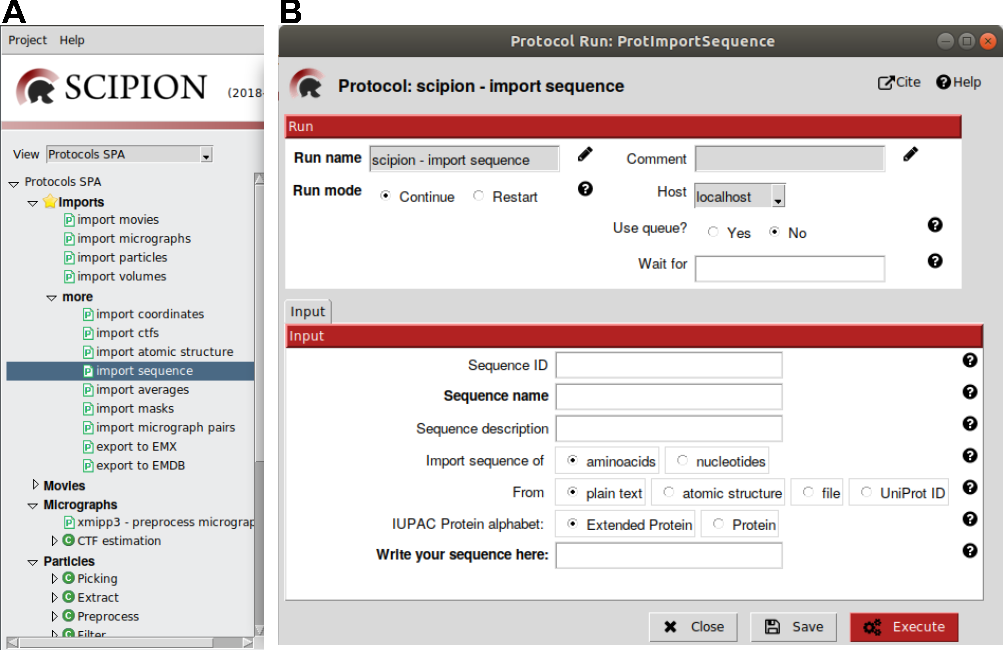
\includegraphics[width=0.90\textwidth]{Images_appendix/Fig104.pdf}
    \caption{Protocol \scommand{import sequence}. A: Protocol location in \scipion menu. B: Protocol form.}
    \label{fig:app_protocol_sequence_1}
   \end{figure}
  
  \begin{itemize}
  \item \ttt{Sequence ID}: Optional short name to identify your sequence (acronym or number, e. g. \ttt{Q05769}). If no ID is assigned by the user, and the sequence has been downloaded from GeneBank/UniProtKB/PDB database, the database ID will be selected as \ttt{Sequence ID} (Read \ttt{Help} section (question mark) to see some examples). Otherwise, \ttt{Sequence name} will be set as \ttt{Sequence ID}.\\
  \item \ttt{Sequence name}: Compulsory short name to identify your sequence (\ttt{PGH2\_MOUSE}). Names with certain meaning are recommended.\\
  \item \ttt{Sequence description}: Optional description of your sequence. It can include functionality, organism, size, etc... (e.g. \ttt{Prostaglandin G/H synthase 2}). If no description is assigned by the user, and the sequence has been downloaded from GeneBank/UniProtKB/PDB database, the database description will be selected as \ttt{Sequence description}. Otherwise, no description will be included.\\
  \item \ttt{Import sequence of}: Selection parameter to choose between \ttt{aminoacids} and \ttt{nucleotides}. After selecting one of them, a new selection menu will be opened:\\
  
  \begin{itemize}
  \item \ttt{aminoacids}: Parameter to select one of these four options:\\
   \begin{itemize}
   \item \ttt{plain text}: Select this option if you want to introduce your own single letter aminoacid sequence. Since your sequence will be cleaned according to the standard protein alphabet of 20 aminoacids (\ttt{Protein}) or to an extended one that includes 6 additional aminoacids or aminoacid groups (\ttt{Extended Protein}), you have to select one of these \ttt{IUPAC Protein} alphabets. Read \ttt{Help} section (question mark) to know the aminoacids included in each alphabet. Not only non-canonical aminoacids will be cleaned, but also wildcard characters such as \ttt{*}, \ttt{\#}, \ttt{?}, \ttt{-}, etc... \ttt{Write your sequence here} indicates the place where your single letter aminoacid sequence has to be written or paste.\\ 
   \item \ttt{atomic structure}: Select this option if you want to download the sequence from an atomic structure (\ffigure{fig:app_protocol_sequence_2} (A)). Select \ttt{id} to download your sequence from PDB database. Then, write the PDB ID (\ttt{Atomic structure ID} and select the chain sequence of your preference (\ttt{Chain}). Use the wizard at the right side of \ttt{Chain} parameter to select that chain. Follow an analogous process to download the sequence from an atomic structure that you already has in your computer. This time, the \ttt{File path} will replace the \ttt{Atomic structure ID}. By pressing the folder symbol, a browser will help you to find the structure file.\\
   \item \ttt{file}: Select this option if your sequence is written in a text file that you already have in your computer (\ffigure{fig:app_protocol_sequence_2} (B)). By pressing the folder symbol, a browser will help you to find the sequence file.\\
   \item \ttt{UniProtID}: Select this option if you want to download the sequence from UniProtKB database (\ffigure{fig:app_protocol_sequence_2} (C)). Write the name/ID of the respective sequence in the parameter box \ttt{UniProt name/ID}. An error message appears in case you introduce a wrong ID.\\
   
   \begin{figure}[H]
    \centering 
    \captionsetup{width=.7\linewidth} 
    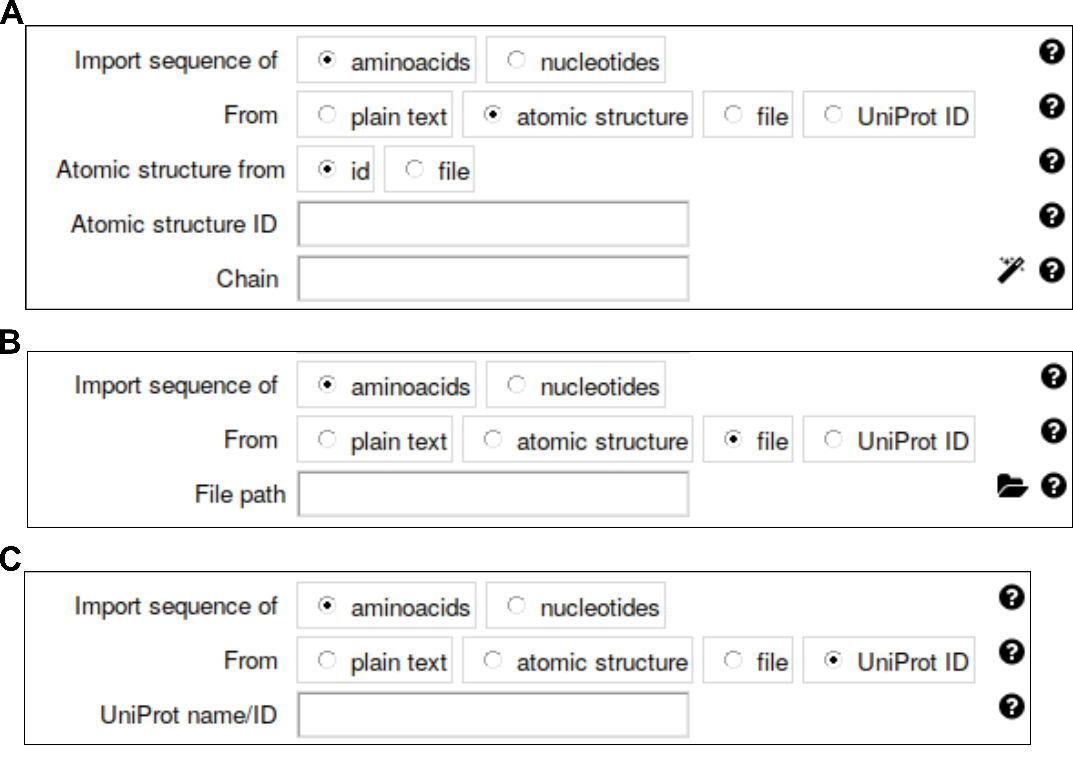
\includegraphics[width=0.90\textwidth]{Images_appendix/Fig105.pdf}
    \caption{Protocol \scommand{import sequence}. Protocol form to import aminoacid sequences from the PDB database by indicating its respective ID (A), from a file (B), or from UniProtKB by writing the database ID/name (C).}
    \label{fig:app_protocol_sequence_2}
   \end{figure}
   
   \end{itemize}
  \item \ttt{nucleotides}: Analogously to \ttt{aminoacids} parameter, select one of these four options:\\
  \begin{itemize}
   \item{plain text}: Parameter to introduce your own single letter nucleotide sequence (\ffigure{fig:app_protocol_sequence_3} (A)). Since your sequence will be cleaned according to the standard nucleic acid alphabet, you have to select one of the next five alphabets. The first three are DNA alphabets and the last two ones are RNA alphabets. Read \ttt{Help} section (question mark) to know each alphabet. The most restricted ones are \ttt{Unambiguous DNA} (``A, C, G, T'') and \ttt{Unambiguous RNA} (``A, C, G, U'') for DNA and RNA, respectively. The cleaning process also involves wildcard characters such as \ttt{*}, \ttt{\#}, \ttt{?}, \ttt{-}, etc...\\
   \item{atomic structure}: Information described for aminoacids is valid for nucleotides (\ffigure{fig:app_protocol_sequence_3} (B)).\\
   \item{file}: Information described for aminoacids is valid for nucleotides (\ffigure{fig:app_protocol_sequence_3} (C)).\\
   \item{GeneBank}: Information described for aminoacids is valid for nucleotides, this time replacing UniProtKB by GeneBank t(\ffigure{fig:app_protocol_sequence_3} (D)).\\
   
   \begin{figure}[H]
    \centering 
    \captionsetup{width=.7\linewidth} 
    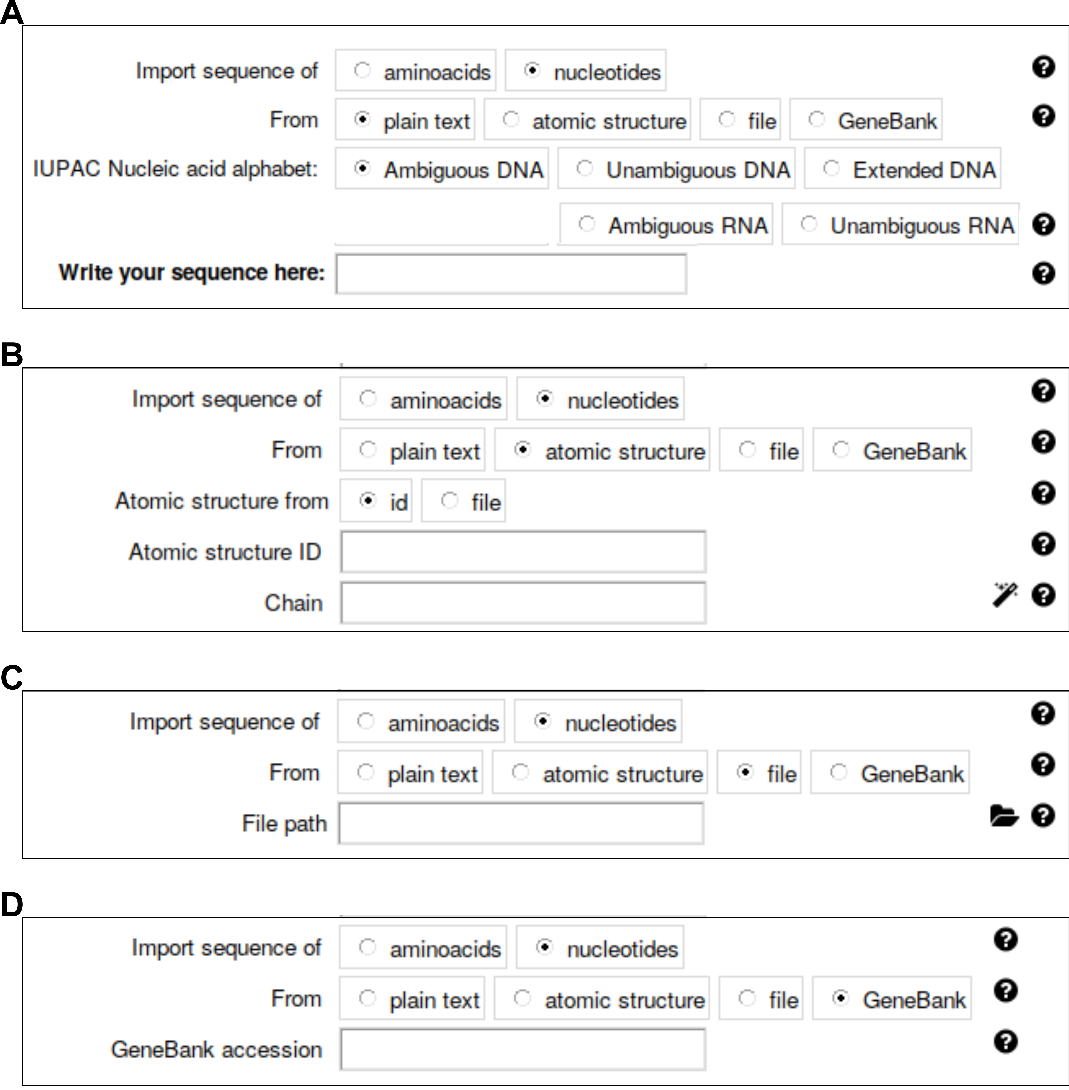
\includegraphics[width=0.90\textwidth]{Images_appendix/Fig106.pdf}
    \caption{Protocol \scommand{import sequence}. Protocol form to write (A) or import nucleotide sequences from PDB database by indicating its respective ID (B), from a file (C), or from GeneBank by writing the database accession number (D).}
    \label{fig:app_protocol_sequence_3}
   \end{figure}
   
  \end{itemize}
  
  \end{itemize}
  

  \end{itemize}
 

  \item Protocol execution:\\

  Adding specific sequence label is recommended in \ttt{Run name} section, at the form top. To add the label, open the protocol form, press the pencil symbol at the right side of \ttt{Run name} box, complete the label in the new opened window, press OK, and finally close the protocol. This label will be shown in the output summary content (see below). If you want to run again this protocol, do not forget to set to \ttt{Restart} the \ttt{Run mode}.\\
  Press the \ttt{Execute} red button at the form bottom.\\
  
  \item Visualization of protocol results:\\
  
  After executing the protocol, press \ttt{Analyze Results} and a text editor will be opened in which you can read the sequence in fasta format. \ttt{Sequence ID} and \ttt{Sequence description} are included in the header.\\ 

 \item Summary content:\\
  \begin{itemize}
     \item Protocol output (below \scipion framework):\\ \ttt{scipion - import sequence  -> ouputSequence}; \ttt{Sequence name}\\
     \item \ttt{SUMMARY} box:\\ Sequence of aminoacids/ nucleotides:\\Sequence \ttt{Sequence name} imported from plain text/ atomic structure/ file/ UniProt ID.\\
    \end{itemize}

  \end{itemize}
